\thispagestyle{timhieukhoahocnone}
\pagestyle{timhieukhoahoc}
\everymath{\color{timhieukhoahoc}}
\blfootnote{$^1$\text{\color{timhieukhoahoc}Chưa có thống nhất về thuật ngữ tiếng Việt cho ``entanglement". Từ này còn được dịch là ``vướng mắc, ``vướng víu",}}
\blfootnote{\text{\color{timhieukhoahoc}``rối", ``ràng buộc".}}
\blfootnote{$^2$\text{\color{timhieukhoahoc}Nguồn: \url{https://www.nobelprize.org/uploads/2022/10/popular-physicsprize2022.pdf.}}}
\blfootnote{\text{\color{timhieukhoahoc}Dịch: Nguyễn Hoàng Thạch (Viện Toán học); hiệu đính: Nguyễn Trần Thuật (ĐHKHTN -- ĐHQG Hà Nội).}}
\graphicspath{{../timhieukhoahoc/pic/}}
\begingroup
\AddToShipoutPicture*{\put(0,616){\includegraphics[width=19.3cm]{../bannertimhieu}}}
\AddToShipoutPicture*{\put(112,542){\includegraphics[scale=1]{../tieude.pdf}}}
\centering
\endgroup
\vspace*{160pt}

\begin{multicols}{2}
	\textit{Bằng những thí nghiệm đột phá, \textbf{\color{timhieukhoahoc}Alain Aspect}, \textbf{\color{timhieukhoahoc}John Clauser} và \textbf{\color{timhieukhoahoc}Anton Zeilinger} đã chỉ ra khả năng nghiên cứu và kiểm soát các hạt ở trạng thái liên đới. Điều xảy đến với một hạt trong một cặp bị liên đới với nhau sẽ quyết định điều xảy đến với hạt còn lại, kể cả khi chúng cách nhau quá xa để có thể tác động đến nhau. Các công cụ thực nghiệm do ba nhà khoa học được giải phát triển đã đặt nền móng cho một kỷ nguyên mới của công nghệ lượng tử.}
%	\vskip 0.1cm
	\begin{figure}[H]
		\vspace*{-5pt}
		\centering
		\captionsetup{labelformat= empty, justification=centering}
		\includegraphics[width= 1\linewidth]{7}
		\vspace*{-20pt}
	\end{figure}
	Những nền tảng cơ bản của cơ học lượng tử không chỉ là vấn đề lý thuyết hay triết học. Nhiều nghiên cứu và phát triển đang diễn ra mạnh mẽ nhằm sử dụng những tính chất đặc biệt của từng hệ hạt riêng rẽ để tạo ra máy tính lượng tử, cải tiến đo lường, xây dựng các mạng lượng tử và thiết lập phương thức truyền tin bảo mật bằng mật mã lượng tử.
	\vskip 0.1cm
	Nhiều ứng dụng phụ thuộc vào cách cơ học lượng tử cho phép hai hay nhiều hạt tồn tại trong cùng một trạng thái, bất kể khoảng cách giữa chúng. Hiện tượng này, được gọi là liên đới lượng tử, là một trong những yếu tố gây tranh luận nhiều nhất trong cơ học lượng tử kể từ khi lý thuyết này được phát biểu. Albert Einstein từng nói về ``tác động ma quái từ xa" và Erwin Schrödinger nói đó là đặc điểm quan trọng nhất của cơ học lượng~tử.
	\vskip 0.1cm
	Các nhà khoa học được giải năm nay đã tìm hiểu các trạng thái liên đới lượng tử này, và các thí nghiệm của họ đã đặt nền móng cho cuộc cách mạng đang diễn ra trong công nghệ lượng tử.
	\vskip 0.1cm
	\textbf{\color{timhieukhoahoc}Khác xa trải nghiệm thường ngày}
	\vskip 0.1cm
	Khi hai hạt ở trong trạng thái liên đới lượng tử, nếu đo được một thuộc tính của một hạt, người ta có thể xác định ngay kết quả của phép đo tương đương đối với hạt còn lại mà không cần phải kiểm tra.
	\vskip 0.1cm
	Thoáng nhìn thì điều này có lẽ không có gì lạ. Nếu nghĩ về những quả bóng thay vì các hạt, ta có thể hình dung một thí nghiệm trong đó quả bóng đen được ném về một hướng, quả bóng trắng được ném về hướng ngược lại. Một người quan sát khi bắt được quả bóng trắng sẽ có thể nói ngay rằng quả bóng được ném theo hướng ngược lại có màu đen.
	\vskip 0.1cm
	Điểm đặc biệt của cơ học lượng tử là những thứ tương đương với những quả bóng (nói ở trên) không có trạng thái xác định cho đến khi chúng được đo. Cứ như thể tất cả bóng đều màu xám, cho tới khi ai đó nhìn vào một quả trong số chúng. Khi đó, quả bóng được quan sát có thể lấy ngẫu nhiên tất cả màu đen hoặc tất cả màu trắng của cả cặp, và quả bóng còn lại lập tức trở thành màu còn lại.
	\vskip 0.1cm
	Nhưng làm sao biết được rằng hai quả bóng không có màu xác định ngay từ đầu? Ngay cả khi chúng đều trông màu xám, biết đâu ẩn bên trong chúng có những nhãn cho biết chúng cần biến thành màu gì khi có người nhìn.
	\vskip 0.1cm
	\textbf{\color{timhieukhoahoc}Màu sắc có tồn tại khi không ai nhìn?}
	\vskip 0.1cm
	Những cặp hạt bị liên đới với nhau trong cơ học lượng tử có thể được ví với một cái máy bắn những quả bóng khác màu về hai hướng ngược nhau. Khi Bob bắt được một quả bóng và thấy rằng nó màu đen, anh ta biết ngay rằng Alice bắt được một quả bóng trắng. Trong một lý thuyết sử dụng những biến ẩn, những quả bóng sẽ luôn chứa thông tin ẩn về màu chúng sẽ hiển thị. Tuy nhiên, cơ học lượng tử nói rằng những quả bóng có màu xám cho tới khi được nhìn, khi đó một quả trở thành màu trắng, một cách ngẫu nhiên, và quả còn lại trở thành màu đen. Các bất đẳng thức Bell chỉ ra rằng có những thí nghiệm có thể phân biệt những trường hợp này. Những thí nghiệm đó đã chứng minh rằng mô tả của cơ học lượng tử là đúng đắn.
	\vskip 0.1cm
	Một phần quan trọng trong những nghiên cứu được trao giải Nobel Vật lý năm nay là hiểu biết lý thuyết sâu sắc có tên gọi \textit{các bất đẳng thức Bell}. Các bất đẳng thức Bell giúp phân biệt được sự bất định của cơ học lượng tử với một mô tả khác sử dụng các \textit{biến ẩn}. Các thí nghiệm cho thấy tự nhiên tuân theo những dự đoán của cơ học lượng tử. Những quả bóng có màu xám, không chứa thông tin bí mật, và việc quả nào trở thành đen, quả nào trở thành trắng là ngẫu nhiên.
	\begin{figure}[H]
		\vspace*{-5pt}
		\centering
		\captionsetup{labelformat= empty, justification=centering}
		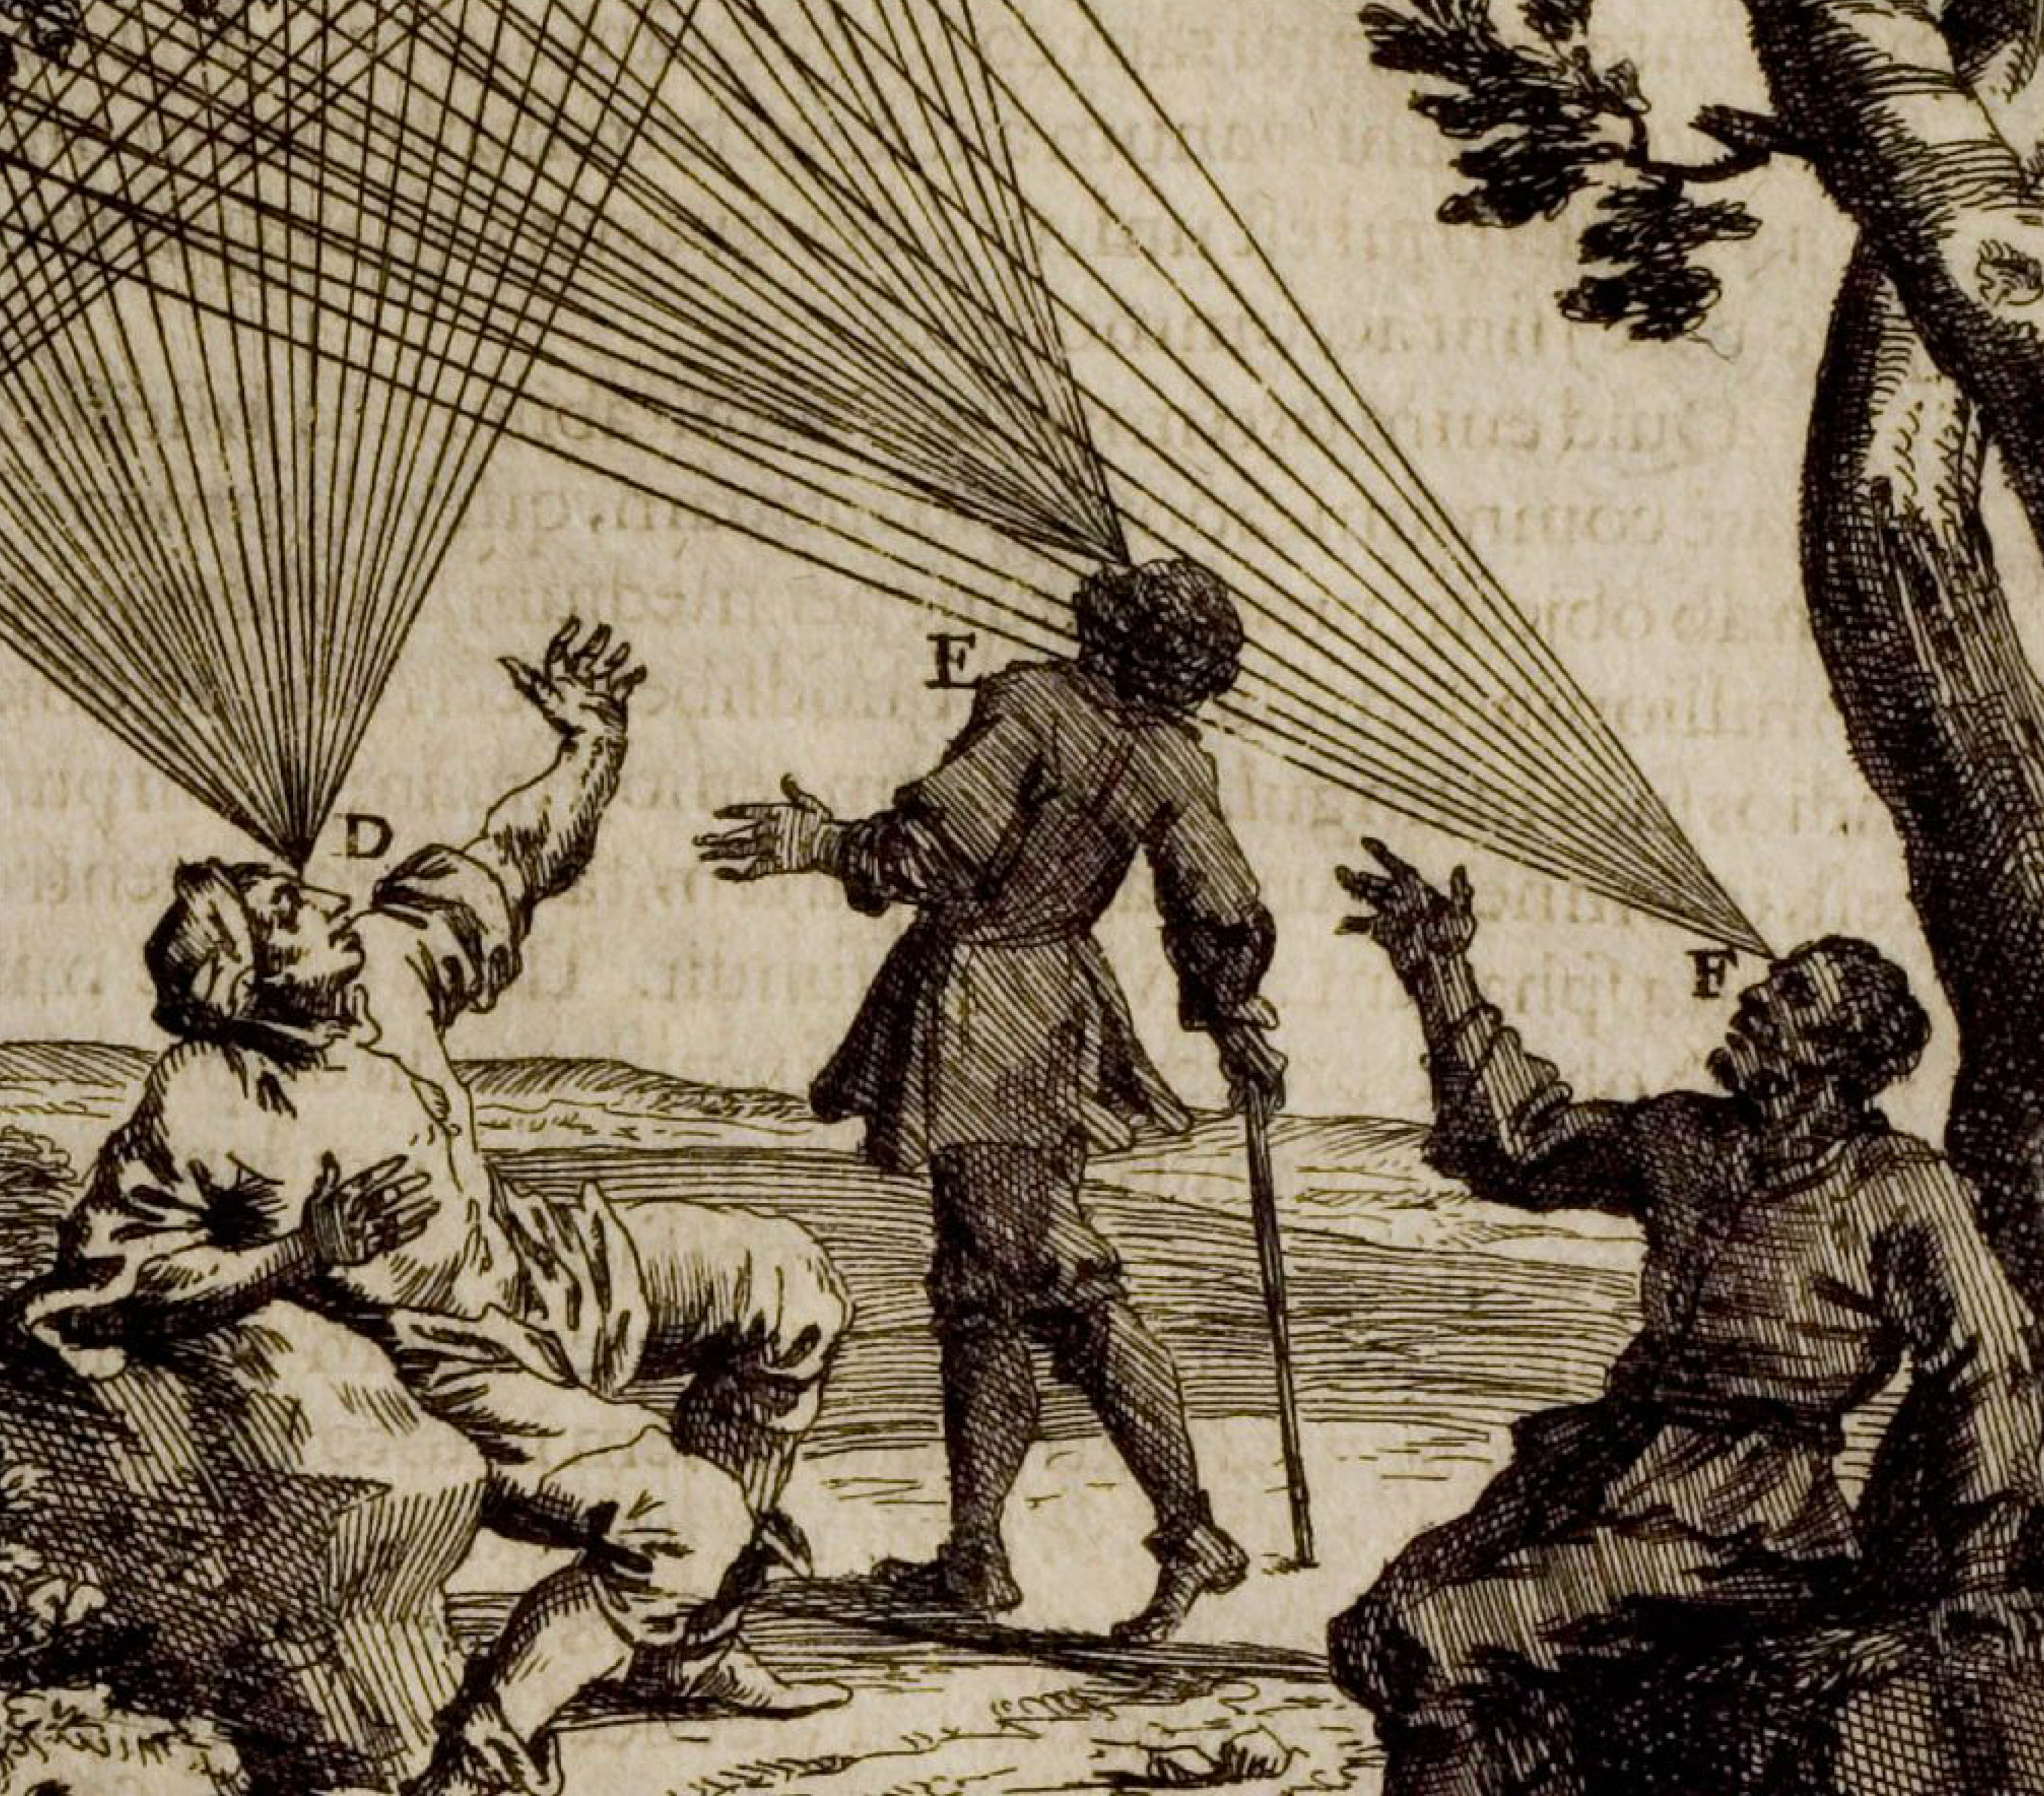
\includegraphics[width= 1\linewidth]{1}
		\caption{\small\textit{\color{timhieukhoahoc}Hình $1$: Biến ẩn.}}
		\vspace*{-10pt}
	\end{figure}
	\begin{figure}[H]
		\vspace*{-5pt}
		\centering
		\captionsetup{labelformat= empty, justification=centering}
		\includegraphics[width= 1\linewidth]{2}
		\caption{\small\textit{\color{timhieukhoahoc}Hình $2$: Cơ học lượng tử.}}
		\vspace*{-10pt}
	\end{figure}
	\textbf{\color{timhieukhoahoc}Tài nguyên quan trọng nhất của cơ học lượng tử}
	\vskip 0.1cm
	Các trạng thái liên đới lượng tử mang lại những phương thức mới tiềm năng để lưu trữ, trao đổi và xử lý thông tin.
	\vskip 0.1cm
	Những điều thú vị xảy ra khi hai hạt trong một cặp liên đới di chuyển theo hai hướng ngược nhau, sau đó một trong chúng gặp một hạt thứ ba và hai hạt này lại trở thành liên đới với nhau. Khi đó, chúng bước vào một trạng thái chung mới. Hạt thứ ba bị mất nhận dạng, nhưng các tính chất ban đầu của nó được chuyển sang hạt lẻ được tách ra từ cặp đầu tiên. Cách truyền một trạng thái lượng tử chưa biết từ một hạt sang một hạt khác như thế này được gọi là \textit{viễn tải lượng tử}. Thí nghiệm kiểu này được thực hiện lần đầu tiên vào năm $1997$ bởi \textbf{\color{timhieukhoahoc}Anton Zeilinger} và các đồng nghiệp.
	\vskip 0.1cm
	Điều đáng chú ý là viễn tải lượng tử là cách duy nhất để truyền thông tin lượng tử từ hệ này sang hệ khác mà không bị thất thoát thông tin. Việc đo tất cả các thuộc tính của một hệ lượng tử rồi chuyển thông tin cho một người nhận để xây dựng lại hệ đó là hoàn toàn không thể. Lý do là một hệ lượng tử có thể chứa đồng thời một vài phiên bản khác nhau của mỗi thuộc tính, mà mỗi phiên bản đều có thể xuất hiện trong một phép đo với một xác suất nhất định. Khi một phép đo được thực hiện, ngay lập tức chỉ còn một phiên bản tồn tại, tức là phiên bản mà thiết bị đo đọc được. Các phiên bản khác biến mất và không có cách nào để biết một chút gì về chúng. Tuy nhiên, những thuộc tính lượng tử hoàn toàn chưa xác định có thể được truyền bằng viễn tải lượng tử và xuất hiện nguyên vẹn ở một hạt khác, đổi lại bằng việc bị phá hủy ở hạt ban đầu.
	\vskip 0.1cm
	Một khi đã chứng minh được điều này bằng thực nghiệm, bước tiếp theo là sử dụng hai cặp hạt liên đới. Nếu một hạt của mỗi cặp được được ghép với nhau theo một cách nào đó, hai hạt còn lại có thể bị liên đới với nhau mặc dù chưa từng tiếp xúc. Sự hoán đổi cặp liên đới này được chứng minh lần đầu tiên vào năm $1998$ bởi nhóm nghiên cứu của Anton Zeilinger.
	\begin{figure}[H]
		\vspace*{-5pt}
		\centering
		\captionsetup{labelformat= empty, justification=centering}
		\includegraphics[width= 1\linewidth]{3}
		\caption{\small\textit{\color{timhieukhoahoc}Hình $3$: Những cặp liên đới chưa từng gặp nhau. Hai cặp liên đới được phát từ hai nguồn khác nhau. Một hạt từ mỗi cặp ($2$ và $3$) được đưa đến với nhau theo một cách nào đó, tạo thành một cặp liên đới. Hai hạt còn lại ($1$ và $4$) cũng sẽ bị liên đới với nhau. Bằng cách này, hai hạt chưa từng tiếp xúc với nhau có thể trở thành bị liên đới với nhau.}}
		\vspace*{-10pt}
	\end{figure}
	Các cặp liên đới gồm hai photon, hạt ánh sáng, có thể có thể được gửi về hai hướng khác nhau theo các sợi quang học và đóng vai trò tín hiệu trong một mạng lượng tử. Các photon chỉ có thể được truyền đi một khoảng cách giới hạn trong sợi quang học trước khi bị hấp thụ hoặc mất các thuộc tính. Tín hiệu quang học thông thường có thể được khuếch đại trên đường truyền, nhưng với các cặp liên đới thì không làm như vậy được. Bộ phận khuếch đại cần thu và đo ánh sáng, do đó sẽ phá hủy trạng thái liên đới. Tuy nhiên, sự hoán đổi cặp liên đới có thể giúp gửi trạng thái ban đầu đi xa hơn, qua đó truyền nó qua những khoảng cách lớn hơn giới hạn trước đó.
	\vskip 0.1cm
	\textbf{\color{timhieukhoahoc}Từ nghịch lý tới bất đẳng thức}
	\vskip 0.1cm
	Bước tiến này dựa trên nhiều năm phát triển. Nó bắt đầu với cái nhìn sâu sắc rằng cơ học lượng tử cho phép một hệ lượng tử riêng lẻ được chia thành nhiều phần tách biệt hẳn nhau nhưng vẫn hoạt động như một thể duy nhất.
	\vskip 0.1cm
	Điều này trái với tất cả những ý tưởng thông thường về quan hệ nhân quả và bản chất của hiện thực. Làm sao mà một thứ có thể bị ảnh hưởng bởi một sự kiện xảy ra ở nơi khác, mà không hề nhận được một dạng tín hiệu nào từ đó? Tín hiệu không thể di chuyển nhanh hơn ánh sáng, nhưng trong cơ học lượng tử, có vẻ như không cần bất cứ một tín hiệu nào để kết nối các phần khác nhau của một hệ rộng lớn.
	\vskip 0.1cm
	Albert Einstein coi điều này là bất khả thi và đã nghiên cứu hiện tượng này cũng với các đồng nghiệp Boris Podolsky và Nathan Rosen. Họ trình bày lập luận của mình vào năm $1935$: cơ học lượng tử có vẻ không cung cấp một mô tả đầy đủ về hiện thực. Điều này về sau được gọi là nghịch lý EPR, theo các chữ cái đầu của tên ba tác giả.
	\vskip 0.1cm
	John Stewart Bell ($1928 - 1990$), nhà vật lý học người Bắc Ai--len làm việc tại CERN, phòng thí nghiệm vật lý hạt của châu Âu, tìm hiểu vấn đề một cách kỹ càng hơn. Ông phát hiện ra rằng có một kiểu thí nghiệm có thể xác định thế giới thuần túy là cơ học lượng tử, hay có một cách mô tả nào khác với những biến ẩn. Nếu thí nghiệm của ông được lặp lại nhiều lần, tất cả các lý thuyết với biến ẩn cho một hệ số tương quan giữa các kết quả, và giá trị này phải nhỏ hơn hoặc bằng một giá trị xác định. Đây chính là bất đẳng thức Bell.
	\vskip 0.1cm
	Tuy nhiên, cơ học lượng tử có thể vi phạm bất đẳng thức này. Nó dự đoán những giá trị hệ số tương quan giữa các kết quả lớn hơn so với những giá trị có thể đạt được với biến ẩn.
	\vskip 0.1cm
	\textbf{\color{timhieukhoahoc}John Clauser} bắt đầu quan tâm đến nền tảng cơ bản của cơ học lượng tử từ khi còn là sinh viên trong những năm $1960$. Sau khi đọc về ý tưởng của John Bell, ông không thể thoát khỏi nó, và cuối cùng, ông cùng với ba nhà khoa học khác đã đề xuất được một kiểu thí nghiệm thực tế để kiểm tra bất đẳng thức Bell.
	\vskip 0.1cm
	Trong thí nghiệm này, một cặp hạt liên đới được đưa về hai hướng ngược nhau. Trong thực tế, thí nghiệm sử dụng các photon với một thuộc tính được gọi là trạng thái phân cực. Khi các hạt được phát ra, hướng phân cực chưa được xác định, điều chắc chắn duy nhất là các hạt có phân cực song song với nhau. Điều này có thể được nghiên cứu bằng cách dùng một kính lọc chỉ cho phép một hướng phân cực nhất định đi qua (Hình $4$). Đây chính là hiệu ứng được dùng trong nhiều loại kính râm để chặn ánh sáng đã bị phân cực tại một bề mặt nào đó, chẳng hạn phản chiếu trên mặt nước.
	\vskip 0.1cm
	Nếu hai hạt trong thí nghiệm được phóng đến hai kính lọc đặt song song với nhau, chẳng hạn cùng thẳng đứng, và một hạt lọt qua, thì hạt còn lại cũng sẽ lọt qua. Nếu hai kính lọc vuông góc với nhau, một hạt bị chặn lại còn hạt kia đi qua. Mẹo ở đây là đo với các kính lọc đặt lệch nhau và theo nhiều hướng khác nhau, vì khi đó có thể có nhiều kết quả khác nhau: khi thì cả hai hạt lọt qua, khi thì chỉ một hạt, khi lại không hạt nào. Tần suất cả hai hạt lọt qua phụ thuộc vào góc giữa hai tấm kính lọc.
	\vskip 0.1cm
	Cơ học lượng tử dẫn đến một mối tương quan giữa các lần đo. Xác suất để một hạt lọt qua phụ thuộc vào góc của tấm kính lọc kiểm tra sự phân cực của hạt còn lại ở phía đối diện của thí nghiệm. Điều này có nghĩa là tại một số góc, kết quả của cả hai phép đo vi phạm bất đẳng thức Bell và có hệ số tương quan lớn hơn giá trị có thể đạt được nếu các kết quả được quyết định bởi biến ẩn và đã được định sẵn từ lúc các hạt được phát ra.
	\vskip 0.1cm
	\textbf{\color{timhieukhoahoc}Bất đẳng thức bị vi phạm}
	\vskip 0.1cm
	John Clauser lập tức bắt tay vào thực hiện thí nghiệm. Ông chế tạo một thiết bị đồng thời phát ra hai photon liên đới với nhau, mỗi photon hướng đến một kính lọc kiểm tra tính phân cực của chúng. Năm $1972$, cùng với nghiên cứu sinh Stuart Freedman ($1944 - 2012$), ông đưa ra được một kết quả cho thấy rõ ràng bất đẳng thức Bell bị vi phạm, và phù hợp với những dự đoán của cơ học lượng tử.
	\vskip 0.1cm
	Trong những năm tiếp theo, John Clauser và các nhà vật lý khác tiếp tục thảo luận về thí nghiệm và những hạn chế của nó. Một trong những hạn chế là thí nghiệm nói chung không hiệu quả, trong cả việc phát lẫn việc thu các hạt. Các phép đo cũng được cố định trước, với các kính lọc gắn cố định. Do đó có những lỗ hổng, theo đó người quan sát có thể nghi ngờ các kết quả: nếu vì lý do nào đó mà thí nghiệm chỉ lựa chọn những hạt có tương quan lớn mà không phát hiện các hạt khác thì sao? Nếu đúng như vậy thì các hạt vẫn có thể mang thông tin ẩn.
	\vskip 0.1cm
	Loại bỏ lỗ hổng này là một việc khó khăn vì các trạng thái liên đới lượng tử rất mong manh và khó điều khiển; cần phải xử lý từng photon riêng. Nghiên cứu sinh người Pháp Alain Aspect không chùn bước, và đã xây dựng một phiên bản thí nghiệm mới mà sau này ông đã tinh chỉnh thêm nhiều lần. Trong thí nghiệm của mình, ông có thể ghi lại những photon nào lọt qua kính lọc và những photon nào thì không. Có nghĩa là nhiều photon được phát hiện hơn, và các kết quả đo tốt hơn.
	\vskip 0.1cm
	Trong phiên bản cuối cùng của các thử nghiệm của mình, ông có thể lái các photon đến hai kính lọc khác nhau đặt ở các góc khác nhau. Sự tinh tế nằm ở một cơ chế đổi hướng các photon trong cặp liên đới sau khi chúng đã được tạo ra và phát đi từ nguồn. Các kính lọc chỉ ở cách sáu mét, do đó sự đổi hướng cần xảy ra trong vài phần tỷ giây. Nếu thông tin photon sẽ đến kính lọc nào ảnh hưởng đến cách photon được phát từ nguồn, photon sẽ không đến kính lọc đó. Thông tin về các kính lọc ở một đầu thí nghiệm cũng không thể truyền đến đầu kia và ảnh hưởng tới các kết quả đo ở đó.
	\vskip 0.1cm
	Bằng cách này, Alain Aspect đã giải quyết một lỗ hổng quan trọng và đưa ra một kết quả rõ ràng: cơ học lượng tử là đúng và không có biến ẩn.
	\vskip 0.1cm
	\textbf{\color{timhieukhoahoc}Kỷ nguyên thông tin lượng tử}
	\vskip 0.1cm
	Những thí nghiệm này và những thí nghiệm tương tự đặt nền móng cho những nghiên cứu mạnh mẽ đang diễn ra trong khoa học thông tin lượng tử.
	\vskip 0.1cm
	Việc có thể điều khiển các trạng thái lượng tử và tất cả các lớp thuộc tính của chúng giúp chúng ta tiếp cận những công cụ có tiềm năng bất ngờ. Đây là cơ sở của tính toán lượng tử, truyền và lưu trữ thông tin lượng tử, và các thuật toán mã hóa lượng tử. Người ta đang sử dụng các hệ có nhiều hơn hai hạt -- tất cả trong trạng thái liên đới -- mà Anton Zeilinger và các đồng nghiệp là những người đầu tiên khám phá.
	\vskip 0.1cm
	Những công cụ ngày càng tinh tế này kéo những ứng dụng thực tế lại ngày càng gần. Người ta đã tạo ra được các trạng thái liên đới lượng tử giữa các photon đi xa hàng chục ki--lô--mét trong sợi quang học, cũng như giữa vệ tinh và trạm trên mặt đất. Trong một thời gian ngắn, các nhà khoa học trên khắp thế giới đã tìm ra nhiều cách sử dụng tính chất mạnh nhất của cơ học lượng tử.
	\vskip 0.1cm
	Cuộc cách mạng lượng tử đầu tiên cho chúng ta transistor và laser, giờ đây chúng ta đang bước vào một kỷ nguyên mới, nhờ những công cụ hiện đại để điều khiển các hệ hạt liên đới.
	\vskip 0.1cm
	\begin{figure}[H]
		\vspace*{-5pt}
		\centering
		\captionsetup{labelformat= empty, justification=centering}
		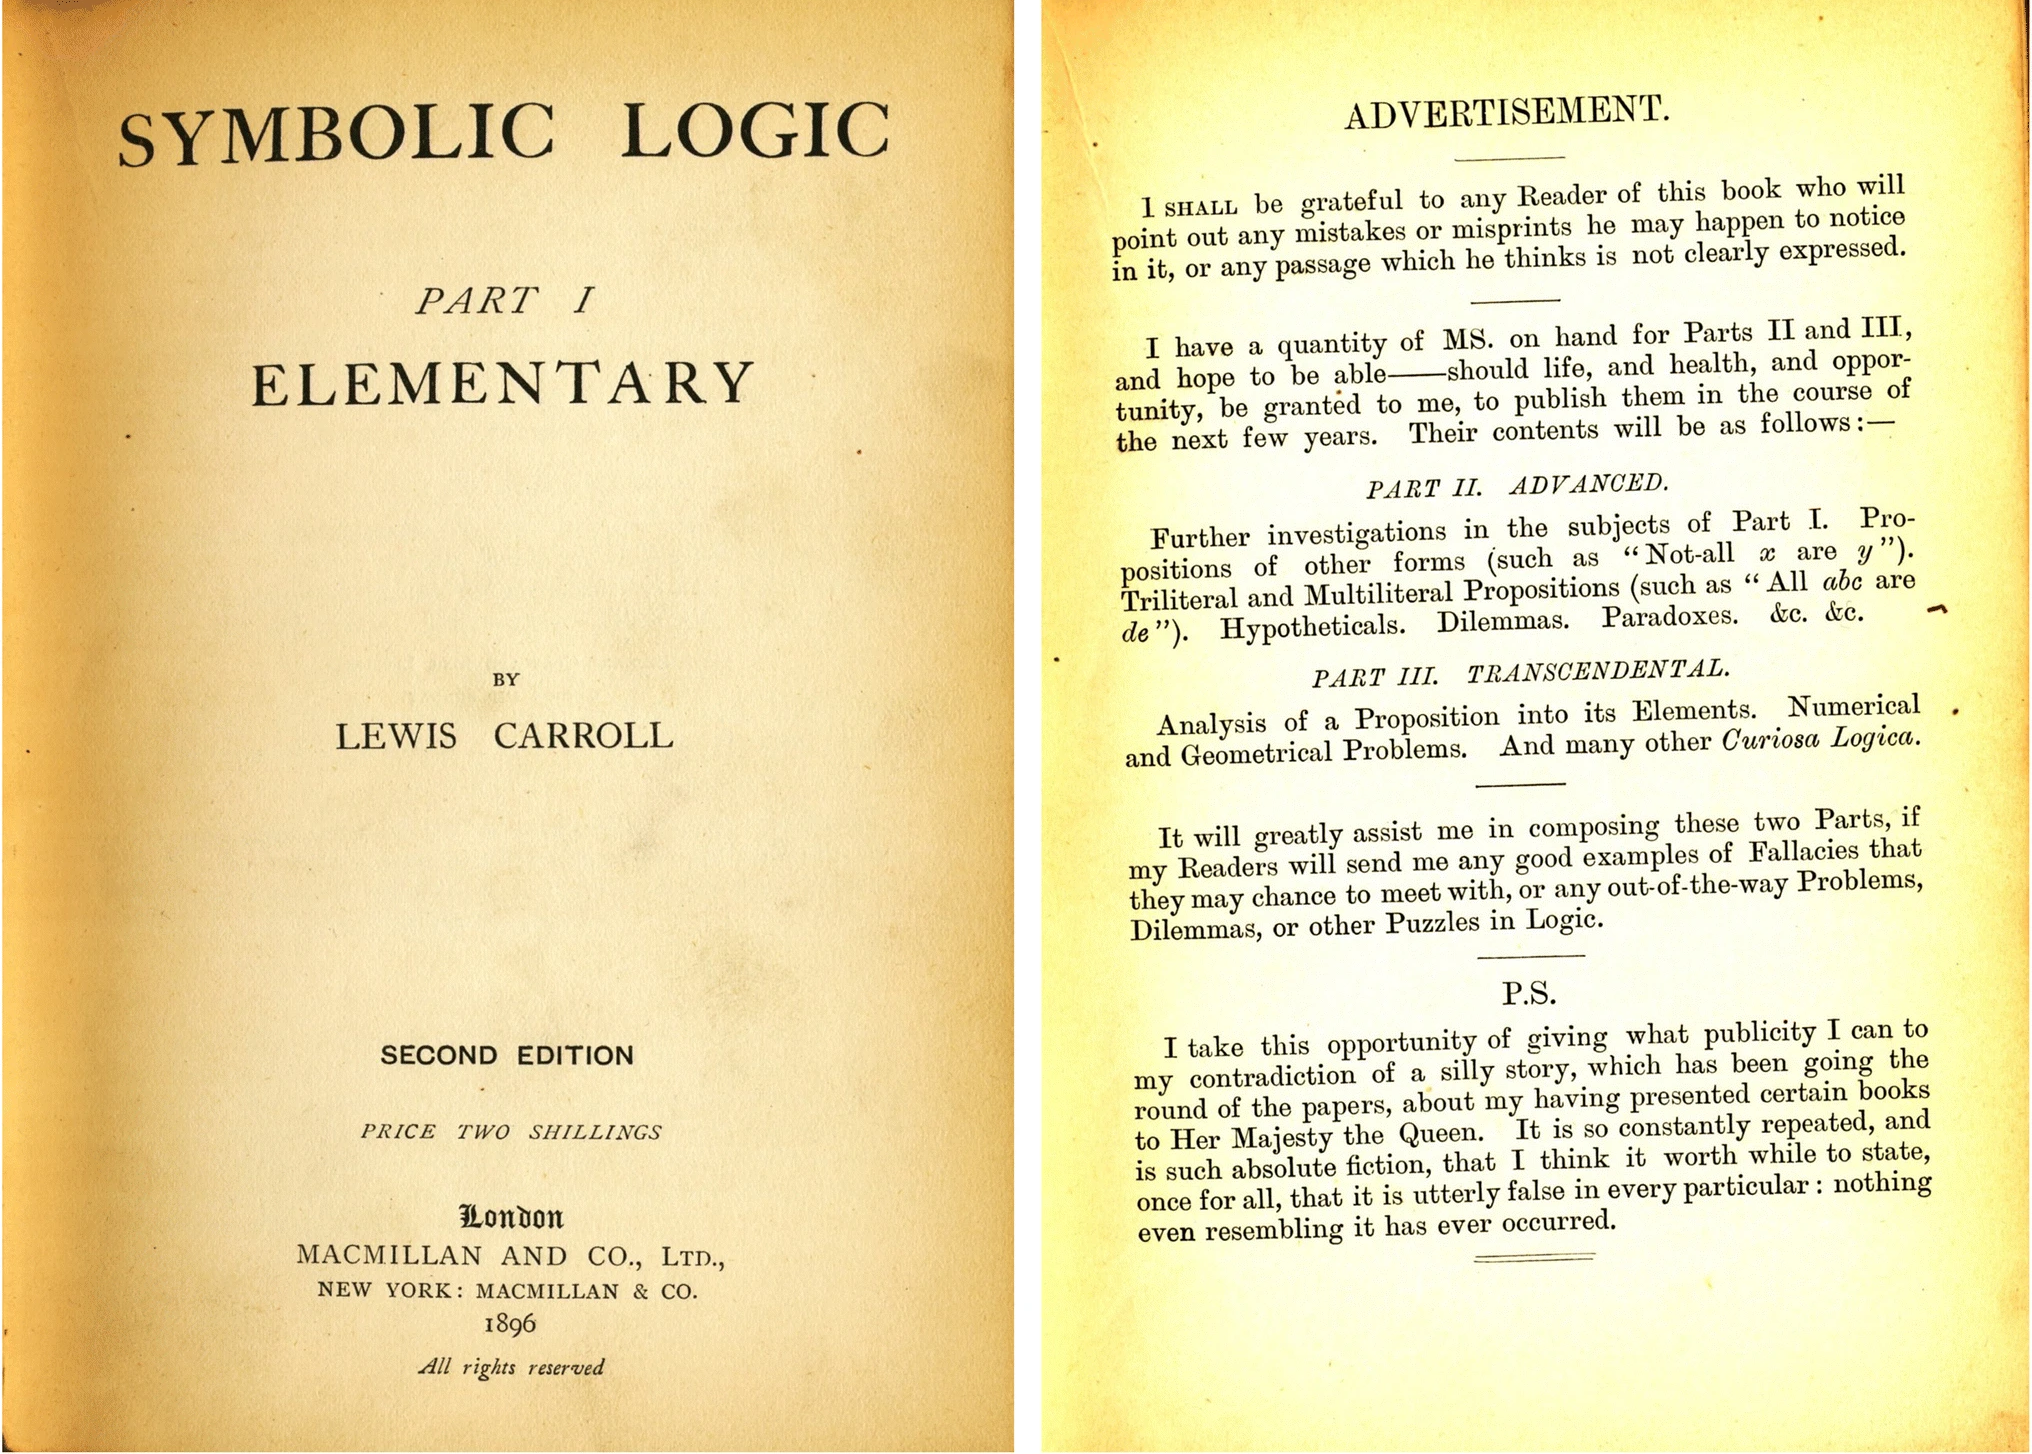
\includegraphics[width= 1\linewidth]{4}
		\caption{\small\textit{\color{timhieukhoahoc}\textbf{\color{timhieukhoahoc}John Clauser} dùng các nguyên tử calcium có thể phát ra các cặp photon liên đới sau khi được một ánh sáng đặc biệt chiếu vào. Ông đặt hai kính lọc ở hai phía để đo sự phân cực của các photon. Sau một loạt các phép đo, ông chứng minh được rằng chúng vi phạm một bất đẳng thức Bell.}}
		\vspace*{-10pt}
	\end{figure}
	\begin{figure}[H]
		\vspace*{-5pt}
		\centering
		\captionsetup{labelformat= empty, justification=centering}
		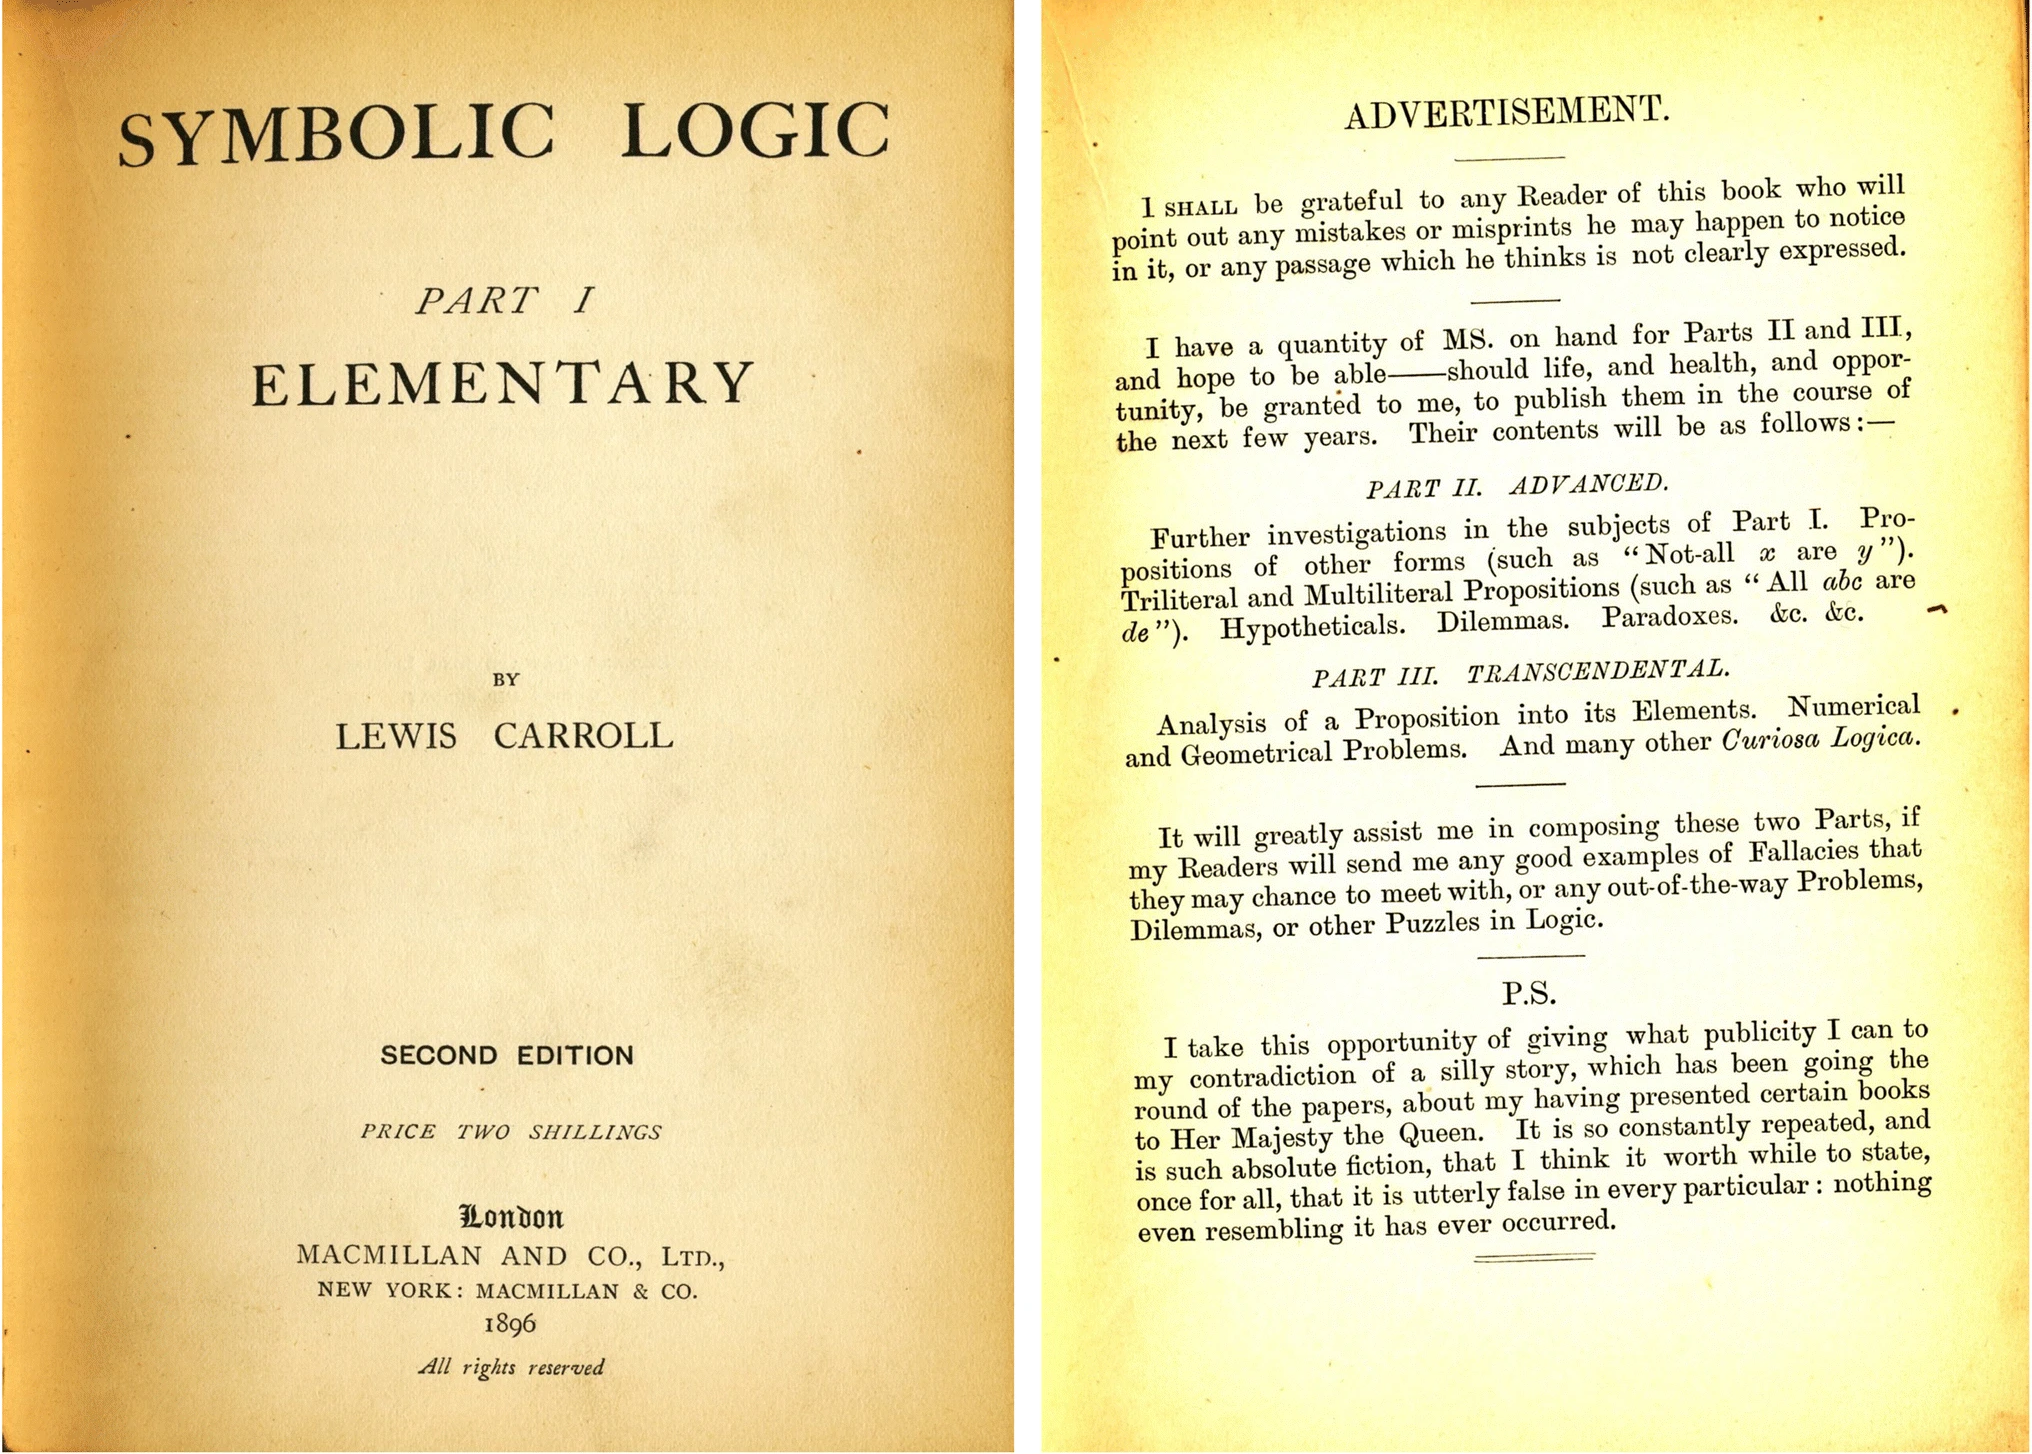
\includegraphics[width= 1\linewidth]{4}
		\caption{\small\textit{\color{timhieukhoahoc}\textbf{\color{timhieukhoahoc}Alain Aspect} phát triển thí nghiệm này, sử dụng một phương pháp mới để kích thích các nguyên tử sao cho chúng phát ra các cặp photon liên đới với tần suất cao hơn. Ông cũng có thể chuyển giữa các thiết lập khác nhau, vì vậy hệ không chứa sẵn một thông tin nào có thể ảnh hưởng đến kết quả.}}
		\vspace*{-10pt}
	\end{figure}
	\begin{figure}[H]
		\vspace*{-5pt}
		\centering
		\captionsetup{labelformat= empty, justification=centering}
		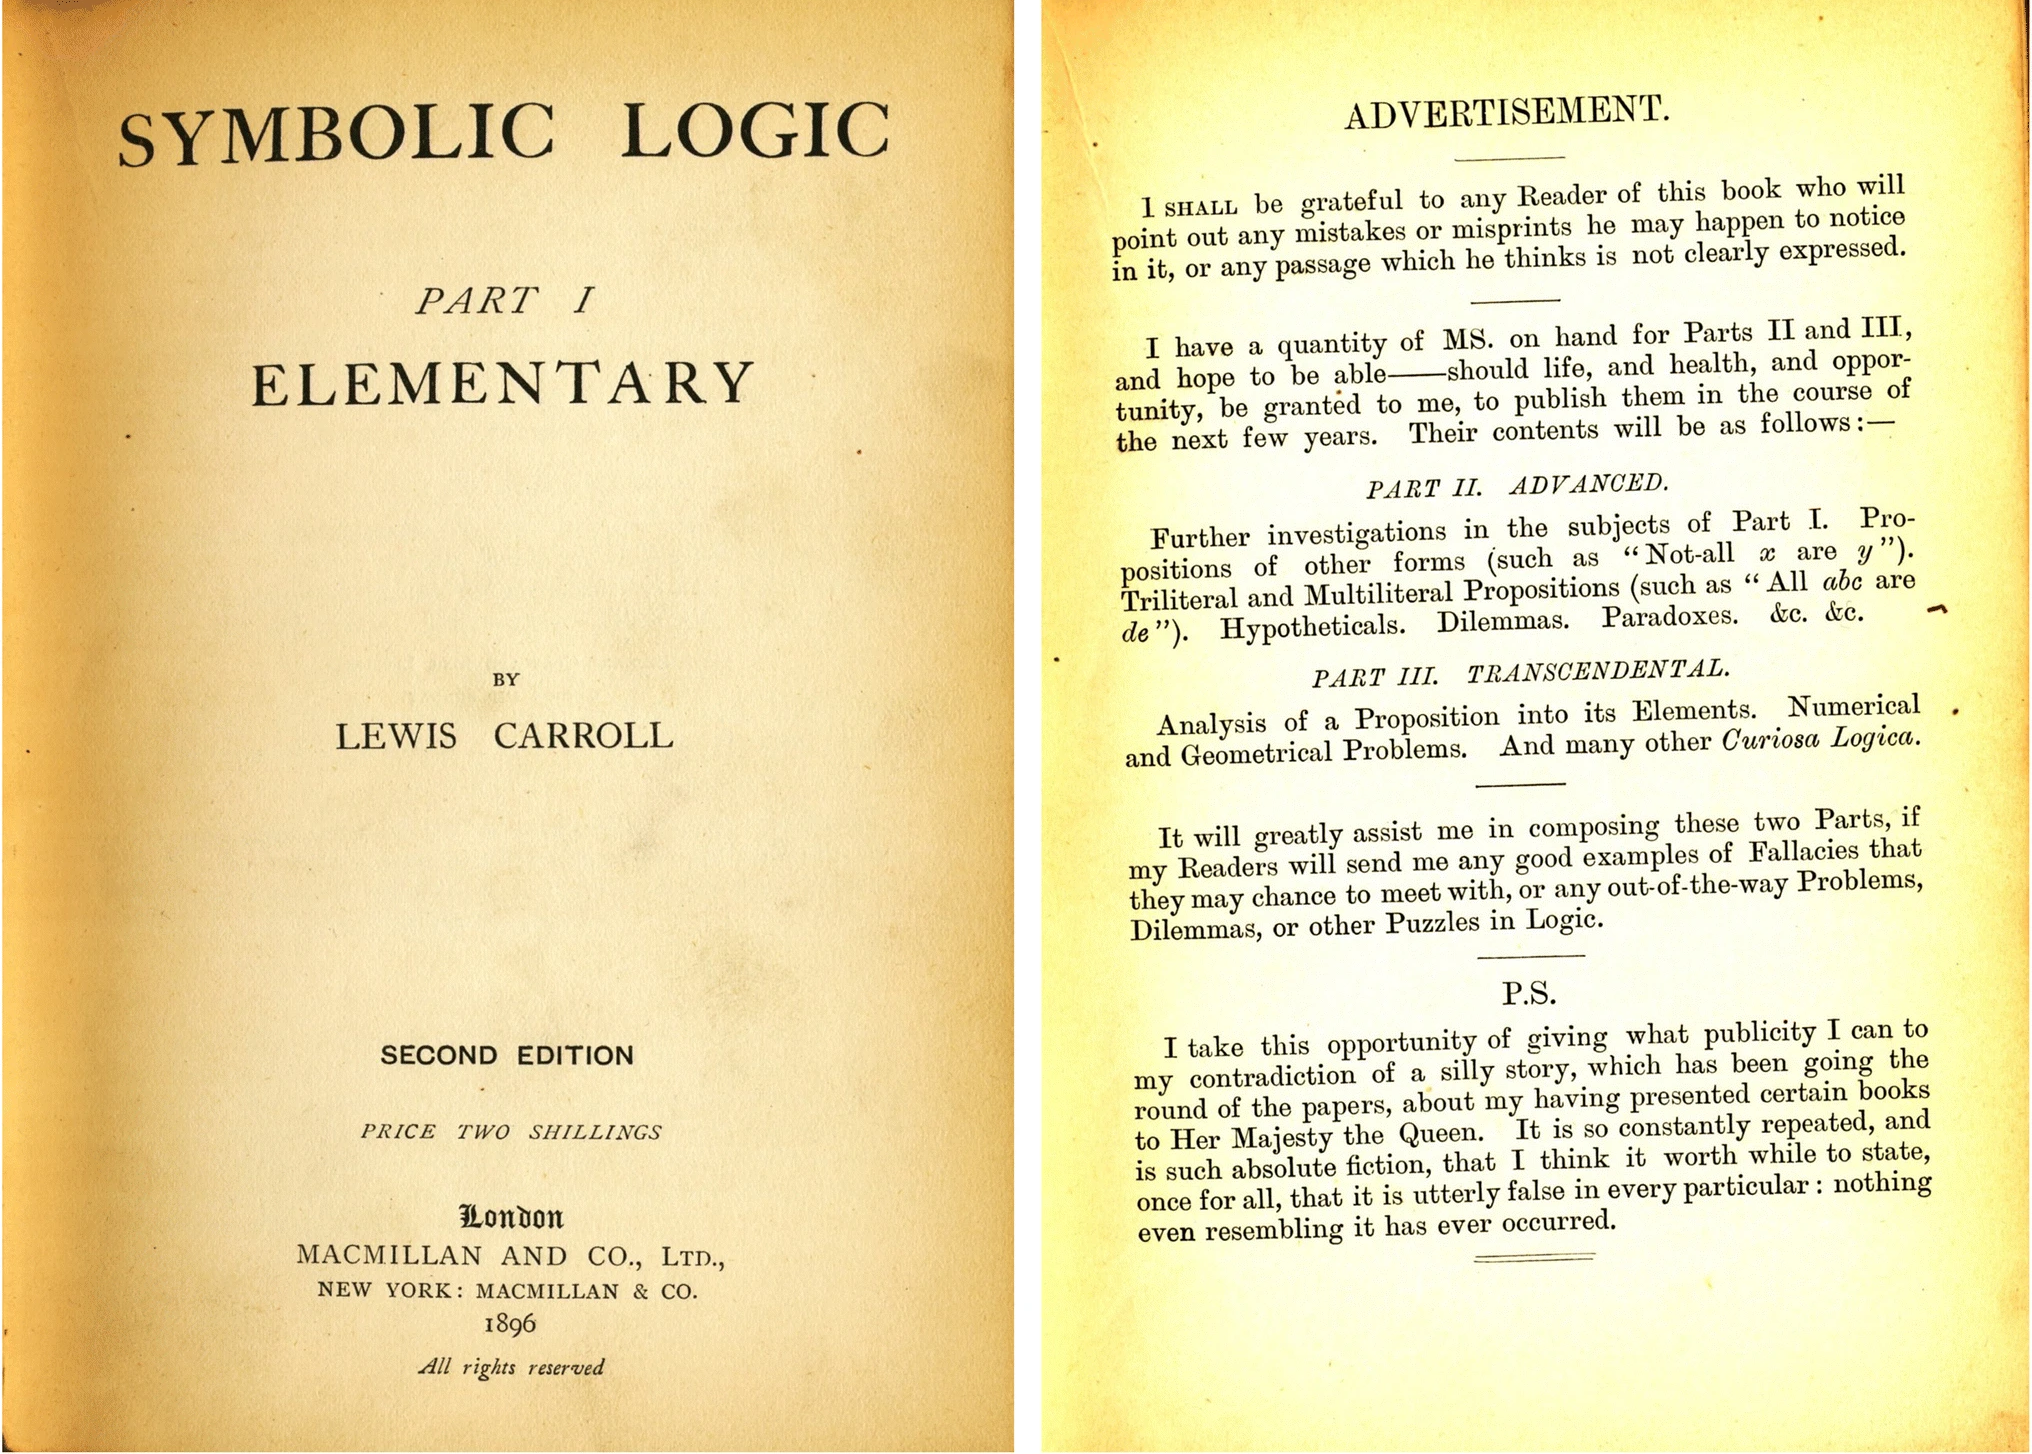
\includegraphics[width= 1\linewidth]{4}
		\caption{\small\textit{\color{timhieukhoahoc}\textbf{\color{timhieukhoahoc}Anton Zeilinger} sau đó thực hiện thêm nhiều thử nghiệm về các bất đẳng thức Bell. Ông tạo ra các cặp photon liên đới bằng cách chiếu một loại laser vào một tinh thể đặc biệt, và sử dụng các số ngẫu nhiên để chuyển giữa các thiết lập đo. Một thí nghiệm sử dụng các tín hiệu từ các thiên hà xa xôi để điều khiển các kính lọc và đảm bảo các tín hiệu không ảnh hưởng lẫn nhau.}}
		\vspace*{-10pt}
	\end{figure}
	\centerline{\small\textit{\color{timhieukhoahoc}Hình $4$: Thí nghiệm với các bất đẳng thức Bell.}}
%	\textbf{\color{timhieukhoahoc}John Clauser} dùng các nguyên tử calcium có thể phát ra các cặp photon liên đới sau khi được một ánh sáng đặc biệt chiếu vào. Ông đặt hai kính lọc ở hai phía để đo sự phân cực của các photon. Sau một loạt các phép đo, ông chứng minh được rằng chúng vi phạm một bất đẳng thức Bell.
	\vskip 0.1cm
%	\textbf{\color{timhieukhoahoc}Alain Aspect} phát triển thí nghiệm này, sử dụng một phương pháp mới để kích thích các nguyên tử sao cho chúng phát ra các cặp photon liên đới với tần suất cao hơn. Ông cũng có thể chuyển giữa các thiết lập khác nhau, vì vậy hệ không chứa sẵn một thông tin nào có thể ảnh hưởng đến kết quả.
%	\vskip 0.1cm
%	\textbf{\color{timhieukhoahoc}Anton Zeilinger} sau đó thực hiện thêm nhiều thử nghiệm về các bất đẳng thức Bell. Ông tạo ra các cặp photon liên đới bằng cách chiếu một loại laser vào một tinh thể đặc biệt, và sử dụng các số ngẫu nhiên để chuyển giữa các thiết lập đo. Một thí nghiệm sử dụng các tín hiệu từ các thiên hà xa xôi để điều khiển các kính lọc và đảm bảo các tín hiệu không ảnh hưởng lẫn nhau.]
\end{multicols}